\documentclass[]{article}
\usepackage{amsmath,amsthm,amssymb,amsfonts}
\usepackage{tikz}
\usepackage{hyperref}

\graphicspath{ {./images/} }

\newtheorem{lemma}{Lemma}
\newtheorem{corollary}{Corollary}
\newtheorem{definition}{Definition}

\renewcommand{\Pr}[1]{\text{Pr}\left(#1\right)} % For probability

\let\oldemptyset\emptyset % Rebind the crappy looking emptyset to another variable
\let\emptyset\varnothing % and redfine emptyset as the good looking one

\newcommand\<{\langle}
\renewcommand\>{\rangle}
\newcommand{\kk}{\ensuremath{\Bbbk}} 
\newcommand{\CC}{\ensuremath{\mathbb{C}}} 
\newcommand{\NN}{\ensuremath{\mathbb{N}}}
\newcommand{\QQ}{\ensuremath{\mathbb{Q}}} 
\newcommand{\RR}{\ensuremath{\mathbb{R}}} 
\newcommand{\ZZ}{\ensuremath{\mathbb{Z}}} 
\newcommand{\cO}{\ensuremath{\mathcal{O}}} 
\newcommand{\Aut}{\ensuremath{\mathrm{Aut}}} 
\newcommand{\Gal}{\ensuremath{\mathrm{Gal}}} 


\newenvironment{solution}
{
	\begin{proof}[Solution] \text{ }
		\\
	}
	{
	\end{proof}
}

%opening
\title{Assignment 3}
\author{Evan Curry Wilbur}

\begin{document}

\maketitle

\subsection*{2.2.2} Each of the following polynomials is written with its monomials ordered according to (exactly) one of lex, grlex, or grevlex order. Determine which monomial order was used in each case.
\begin{enumerate}
	\item[a.] $f(x, y, z) = 7x^2y^4z - 2xy^6 + x^2y^2$
	\item[b.] $f(x, y, z) = xy^3z + xy^2z^2 + x^2z^3$
	\item[c.] $f(x, y, z) = x^4y^5z + 2x^3y^2z - 4xy^2z^4$
\end{enumerate}
\begin{solution}
	\begin{enumerate}
		\item[a.] grlex
		\item[b.] grevlex
		\item[c.] lex
	\end{enumerate}
\end{solution}

\subsection*{2.2.3} Rewrite each of the following polynomials, ordering the terms using the lex order, the grlex order, and the grevlex order, giving $\text{LM}(f), \text{LT}(f),$ and $\text{multideg}(f)$ in each case when the variables are ordered $z > y > x$
\begin{enumerate}
	\item[a.] $f(x, y, z) = 2x + 3y + z + x^2 -z^2 + x^3$
	\item[b.] $f(x, y, z) = 2x^2y^8 - 3x^5yz^4 + xyz^3 - xy^4$
\end{enumerate}
\begin{solution}
\begin{enumerate}
	\item[a.] \text{ } \\
	\begin{tabular}{l|r|r|r}
		 & Lex & Grlex & Grevlex \\
		\hline
		Polynomial & $x^3 + x^2 + 2x + 3y - z^2 + z$ & $x^3 + x^2- z^2 + 2x + 3y + z$ & $x^3 + x^2 - z^2 + 2x + 3y  + z$\\
		$\text{LM}(f)$ & $x^3$ & $x^3$ & $x^3$\\
		$\text{LT}(f)$ & $x^3$ & $x^3$ & $x^3$\\
		$\text{multideg}(f)$ & $(3,0,0)$ & $(3,0,0)$ & $x^3$
	\end{tabular}
	\item[b.] \text{ } \\
	\begin{tabular}{l|r|r|r}
		& Lex & Grlex & Grevlex \\
		\hline
		Polynomial & & & \\
		$\text{LM}(f)$ & & & \\
		$\text{LT}(f)$ & & & \\
		$\text{multideg}(f)$ & & &
	\end{tabular}
\end{enumerate}
\end{solution}

\subsection*{2.2.5} Show that grevlex is a monomial order according to Definition 1.
\begin{solution}
	\begin{definition}
		Let $S$ be some set, $(T, \sim)$ be a partial order and $f : S \to T$ be an injective function. The relation $\sim' \subseteq S \times S$ defined by
		$$
			x \sim' y \iff 
		$$
	\end{definition}
	\begin{lemma}
		Let $\left(S, \leq\right)$ and $\left(T, \preceq\right)$ be two partial orders and $f : S \to T$ be an order embedding such that for all $\alpha, \beta \in S, f(\alpha + \beta) = f(\alpha) + f(\beta)$. Then if $T$ is a monomial ordering, so is $S$.
		%Then $S$ is a monomial ordering only when $T$ is a monomial ordering.
	\end{lemma}
	\begin{proof}
		Let the above be given and suppose $T$ is a monomial ordering. First, we show that $\left(S, \leq\right)$ is a total ordering. Indeed, given some $\alpha, \beta \in S$, since $\left(T, \preceq\right)$ is total, one and only one of the following must be true
		\begin{enumerate}
			\item $f(\alpha) < f(\beta)$
			\item $f(\alpha) > f(\beta)$
			\item $f(\alpha) = f(\beta)$.
		\end{enumerate}
		In any of these three cases, \href{https://en.wikipedia.org/wiki/Order_embedding}{by definition of an order embedding}, the corresponding relation must be true. That is to say, if $f(\alpha) < f(\beta)$ then it must be the case that $\alpha < \beta$, and correspondingly for the remaining two possibilities. Thus $S$ is totally ordered.
		\\
		\\
		Next, we show that $S$ is well-ordered. Let $A \subseteq S$ be some non-empty subset. Since $f(A) \subseteq T$ and $T$ is well ordered, there must exist a smallest element $t \in f(A)$. Necessarily, since every order embedding is injective, there must exist a unique element $a \in A$ such that $f(a) = t$. It will be shown that $a$ is the smallest element of $A$. Indeed if there were to exist some $a' \in A$ such that $a' < a$ then $f(a') < f(a) = t$, contradicting the fact that $t$ is the smallest element of $f(A)$. Hence $\left(S, \leq\right)$ is well-ordered.
		\\
		\\
		Finally, we show that if $\alpha, \beta, \gamma \in A$ with $\alpha > \beta$ then $\alpha + \gamma > \beta + \gamma$. Again by definition of an order embedding, we must have $f(\alpha) > f(\beta)$. Additionally, $f(\gamma) \in T$ and since $T$ is a monomial ordering it follows that
		\begin{align*}
			f(\alpha) + f(\gamma) &> f(\beta) + f(\gamma) &&\implies \\
			f(\alpha + \gamma) &> f(\beta + \gamma) &&\implies \\
			\alpha + \gamma &> \beta + \gamma.
		\end{align*}
		Thus $(S, \leq)$ is a monomial ordering.
	\end{proof}
	
\end{solution}

\subsection*{2.2.6} Another monomial order is the \textbf{inverse lexicographic} or \textbf{invlex} order defined by the following: for $\alpha, \beta \in \ZZ_{\geq 0}^{n}, \alpha >_{\text{invlex}} \beta$ if and only if the rightmost nonzero entry of $\alpha - \beta$ is positive. Show that invlex is equivalent to the lex order with the variables permuted in a certain way. (Which permutation?)

\subsection*{2.3.5} We will study the division of $f = x^3 - x^2y - x^2z + x$ by $f_1 = x^2y-z$ and $f_2 = xy - 1$. 
\begin{enumerate}
	\item[a.] Compute using grlex order:
	\begin{align*}
		r_1 &= \text{remainder of $f$ on division by $\left(f_1, f_2\right)$.} \\
		r_2 &= \text{remainder of $f$ on division by $\left(f_2, f_1\right)$.}
	\end{align*}
	Your results should be \textit{different}. Where in the division algorithm did the difference occur?
	\item[b.] Is $r = r_1 - r_2$ in the ideal $\<f_1, f_2\>$? If so, find an explicit expression $r = Af_1 + Bf_2$. If not, say why not.
	\item[c.] Compute the remainder of $r$ on division by $\left(f_1, f_2\right)$. Why could you have predicted your answer before doing the division?
	\item[d.] Find another polynomial $g \in \<f_1, f_2\>$ such that the remainder on division of $g$ by $(f_1, f_2)$ is nonzero. Hint: $(xy + 1)\cdot f_2 = x^2y^2 - 1$, whereas $y\cdot f_1 = x^2y^2-yz$
	\item[e.] Does the division algorithm give us a solution for the ideal membership problem for the ideal $\<f_1, f_2\>$? Explain your answer
\end{enumerate}
\begin{solution}
	\begin{enumerate}
		\item[a.] On a separate sheet of paper, I computed the remainder to be
		\begin{align*}
			r_1 &= x^3 - x^2z + x - z \\
			r_2 &= x^3 - x^2z
		\end{align*}
		\item[b.] Yes
		$$
			r = -\left(x^2y - z\right) - x\left(xy - 1\right)
		$$
		\item[c.] There is no need to compute the remainder since it must be $r = x - z$. This can be readily seen since neither $\text{LT}(f_1)$ or $\text{LT}(f_2)$ divide any of the terms in $r$. 
		\item[d.] The polynomial $g = yz - 1 \in \<f_1, f_2\>$, but the remainder on division of $g$ by $(f_1, f_2)$ is $-1$.
		\item[e.] No, even if a polynomial $g \in \<f_1, f_2\>$, it need not be the case that the remainder of $g$ by $(f_1, f_2)$ is zero.
	\end{enumerate}
\end{solution}

\subsection*{2.3.9} The discussion around equation (2) of Chapter 1, \S4 shows that every polynomial $f \in \RR[x,y,z]$ can be written as
$$
	f = h_1\left(y - x^2\right) + h_2\left(z-x^3\right) + r,
$$
where $r$ is a polynomial in $x$ alone and $\textbf{V}\left(y-x^2, z-x^3\right)$ is the twisted cubic curve in $\RR^3$.
\begin{enumerate}
	\item[a.] Give a proof of this fact using the division algorithm. Hint: You need to specify carefully the monomial ordering to be used. 
	\item[b.] Use the parametrization of the twisted cubic to show that $z^2 - x^4y$ vanishes at every point of the twisted cubic.
	\item[c.] Find an explicit representation 
	$$
		z^2 - x^4y = h_1\left(y - x^2\right) + h_2\left(z - x^3\right)
	$$
	using the division algorithm.
\end{enumerate}

\subsection*{2.3.10} Let $V \subseteq \RR^3$ be the curve parametrized by $\left(t, t^m, t^n\right), n, m \geq 2.$
\begin{enumerate}
	\item[a.] Show that $V$ is an affine variety.
	\item[b.] Adapt the ideas in Exercise 9 to determine $\textbf{I}(V)$.
\end{enumerate}

\subsection*{2.4.3} Let $I = \<x^6, x^2y^3,xy^7\> \subseteq k[x,y].$
\begin{enumerate}
	\item[a.] In the $(m, n)\text{-plane}$, plot the set of exponent vectors $\left(m,n\right)$ of monomials $x^my^n$ appearing in elements of $I$.
	\item[b.] If we apply the division algorithm to an element $f \in k[x,y]$, using the generators of $I$ as divisors, what terms can appear in the remainder?
\end{enumerate}
\subsection*{2.4.4} Let $I \subseteq k[x,y]$ be the monomial ideal spanned over $k$ by the monomials $x^\beta$ corresponding to $\beta$ in the shaded region shown at the top of the next page.
\begin{enumerate}
	\item[a.] Use the method given in the proof of Theorem 5 to find an ideal basis for $I$.
	\item[b.] Find a minimal basis for $I$ in the sense of Proposition 7.
\end{enumerate}
\begin{center}
	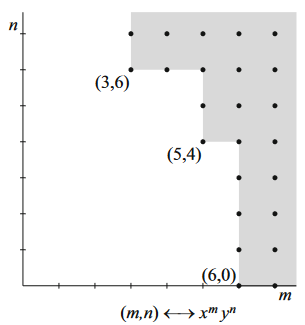
\includegraphics{2-4-4.png}
\end{center}

\subsection*{2.4.9} Suppose we have the polynomial ring $k[x_1,\dots,x_n,y_1,\dots,y_m]$. Let us define a monomial order $>_\text{mixed}$ on this ring that mixes lex order for $x_1,\dots,x_n$, with grlex order for $y_1,\dots,y_m$. If we write monomials in the $n + m$ variables as $x^{\alpha}y^{\beta}$, where $\alpha \in \ZZ_{\geq 0}^n$ and $\beta \in \ZZ_{\geq 0}^{m}$, then we define
$$
	x^{\alpha}y^{\beta} >_{\text{mixed}} x^{\gamma}y^{\delta} \iff x^{\alpha} >_{\text{lex}} x^{\gamma} \text{ or } x^{\alpha} = x^{\gamma} \text{ and } y^{\beta} >_{\text{grlex}}y^\delta.
$$
Use Corollary 6 to prove that $>_\text{mixed}$ is a monomial order. This is an example of what is called a \textit{product order}. It is clear that many other monomial orders can be created by this method.

\subsection*{2.5.1} Let $I = \<g_1,g_2,g_3\> \subseteq \RR[x,y,z]$, where $g_1 = xy^2 - xz + y, g_2 = xy - z^2$ and $g_3 = x - yz^4$. Using the lex order, give an example of $g \in I$ such that $\text{LT}(g) \notin \<\text{LT}(g_1), \text{LT}(g_2), \text{LT}(g_3)\>$.

\subsection*{2.5.7} If we use grlex order with $x > y > z$, is $\{x^4y^2-z^5,x^3y^3-1,x^2y^4-2z\}$ a Gröbner basis for the ideal generated by these polynomials? Why or why not?

\subsection*{2.5.8} Repeat Exercise 7 for $I = \<x - z^2, y - z^3\>$ using the lex order. Hint: The difficult part of this exercise is to determine exactly which polynomials are in $\<LT(I)\>$

\subsection*{2.5.9} Let $A = (a_{ij})$ be an $m \times n$ matrix with real entries in row echelon form and let $J \subseteq \RR[x_1 , . . . , x_n ]$ be an ideal generated by the linear polynomials $\sum_{j=1}^{n}  a_{ij} x_j for 1 \leq i \leq m$.
Show that the given generators form a Gröbner basis for J with respect to a suitable
lexicographic order. Hint: Order the variables corresponding to the leading 1’s before
the other variables

\end{document}
